\section{Lösungsansatz} 

Client 1 hat vom Server Client 2 bis Client 7 als Nachbarn zugewiesen bekommen (Abbildung~\ref{clientkartelegenablauf}). Als erstes selektiert der Client 1 eine Karte und versucht diese bei sich selbst Legen. Gelingt dies nicht, versucht er die Karte bei einem seiner 6 Nachbarn zu legen, indem er ihnen die Karte übergibt und, falls sie gelegt werden konnte, eine Erfolgsmeldung (\textit{true}) oder ansonsten eine Misserfolgsmeldung (\textit{false}) zurückbekommt. Konnte er die selektierte Karte legen, wird diese gelöscht und eine neue Karte wird selektiert, mit welcher wieder von vorne begonnen wird. Das Beispiel von Client 1 ist representativ für alle Clients. 

\begin{figure}[hbt]
  \centering
  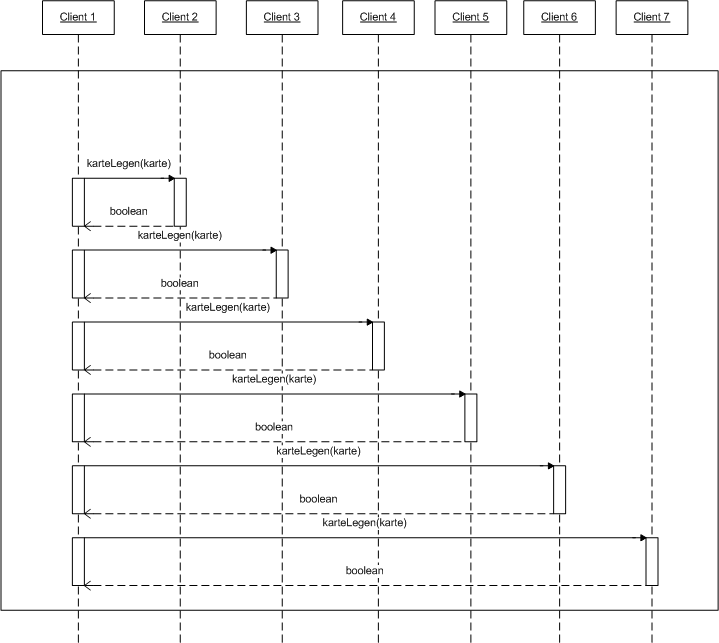
\includegraphics[width=0.90\textwidth,angle=0]{graphics/Kartenlegen_Sequenzdiagramm.png}
  \caption{Sequenzdiagramm: Kartenlegen}
  \label{clientkartelegenablauf}
\end{figure}

Dadurch, dass nicht zuerst der Status der Spiel-Stapel der Nachbarn abgefragt werden muss und danach versucht wirde eine Karte zu lege, ist die Kommunikation auf den Versuch einfach eine Karte zu legen minimiert. Es wird also nur eine Karte übertragen und entweder "true" für den Erfolg oder "false" für den Misserfolg zurückgegeben.
Zudem verwaltet jeder Spieler (Client) seine eigenen Spiel-Stapel vor sich. Diejenigen die er selbst erstellt hat mit einer Eins. Der Spieler muss also nur maximal 4 Spiel-Stapel verwalten auf die andere Spieler (Clients) Zugriff haben. 
Auch ist die anzahl Spieler die auf diese Spiel-Stapel Zugriff haben beschränkt, indem jeder Spieler nur 6 Nachbarn bekommt, mit denen er spielen kann. Wenn diese Nachbarn Sinnvoll verteilt sind, also das heisst solche Spieler die Lokalisationsmässig nahe beieinander liegen auch Nachbarn sind, findet die Kommunikation nur lokal statt und somit wirde ebenfalls die Kommunikation über das globale Netz minimiert.
% Bewertungsmasstab:
% - Ist der Algorithums zur Lösung der Teilafugaben nachvollziehbar? (3 Punkte)

%    - Der Teil für die Initialisierung/Setup wird nicht hier bewertet
%    - 2 Punkte für die komplexeren Komponenten (z.B. die "Clients")
%    - 1 Punkt für die weniger komplexen Komponenten
%    - Das umfasst auch die Kommunikation (wann kommuniziert wer mit wem)

% Nutzung der Ressourcen / Performance
%  -  Ist die Kommunikation minimiert?
%  -  Ist der Bedarf an Memory / Storage sinnvoll?